\section{second closed-loop simulation}

\subsection{Simulink diagram}
	Figure~\ref{fig: simulink diagram main} contains the Simulink diagram for the second closed loop system. Just as with the Simulink diagram in the previous section a subsystem was used for the linear system(figure~\ref{fig: simulink diagram lin system LQR2} ). This time however the internal states where not used by the controller, but as a way to measure how good the estimation of the state is. 
	
	The estimator(figure~\ref{fig: simulink estimator}) contains a simple low pass filter on frequency $f_c$. The filter is followed by a simple discrete finite difference operator. This will result in the measurement of $\dot{\alpha}$ and $\dot{\theta}$. $\theta$ and $\alpha$ itself can be measured directly.
	
	The controller might produce inputs on the motor of over 5 voltage. This obviously cannot be allowed to enter the linear system. That is why the saturation element was used, the motors voltage limits is between $\pm 5V$, and so this is also the maximum and minimum voltage used in the saturation element.
	
	The sample frequency was set at $f_s=200Hz$ which is the same as with the physical system. The estimator contains an ADC which has an $f_s$ of 200Hz and so the controller will only change its outputs at a frequency of 200Hz.
	
	The noise was added after the linear system and before the estimator. This means that the estimated states will contain noise. The power in noise is equal to the variance of the measured noise. This is further explained in the next section. Where the actual measurements are taking place, there it will become clear that the noise is close to Gaussian white noise.

	\begin{figure}[H]
		\centering
		\begin{subfigure}[b]{0.7\textwidth}
			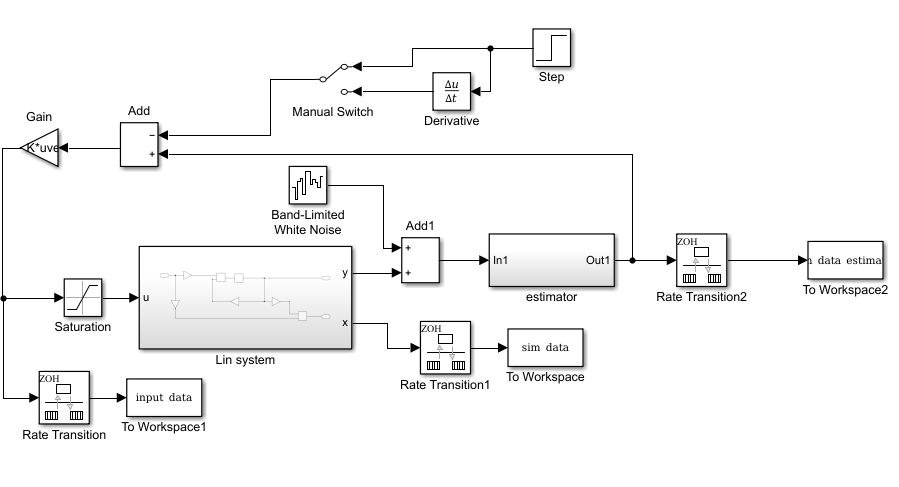
\includegraphics[width=\textwidth]{./part3_LQR2/not_generated/simulink_main.png}
			\caption{main diagram simulink}
			\label{fig: simulink diagram main}
		\end{subfigure}
		\begin{subfigure}[b]{0.45\textwidth}
			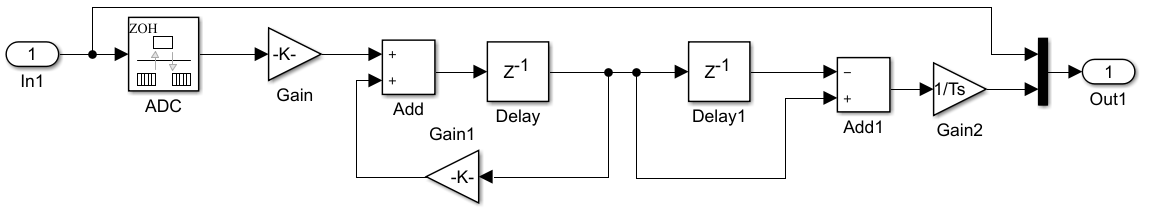
\includegraphics[width=\textwidth]{./part3_LQR2/not_generated/simulink_estimator.png}
			\caption{estimator}
			\label{fig: simulink estimator}
		\end{subfigure}
		\begin{subfigure}[b]{0.45\textwidth}
			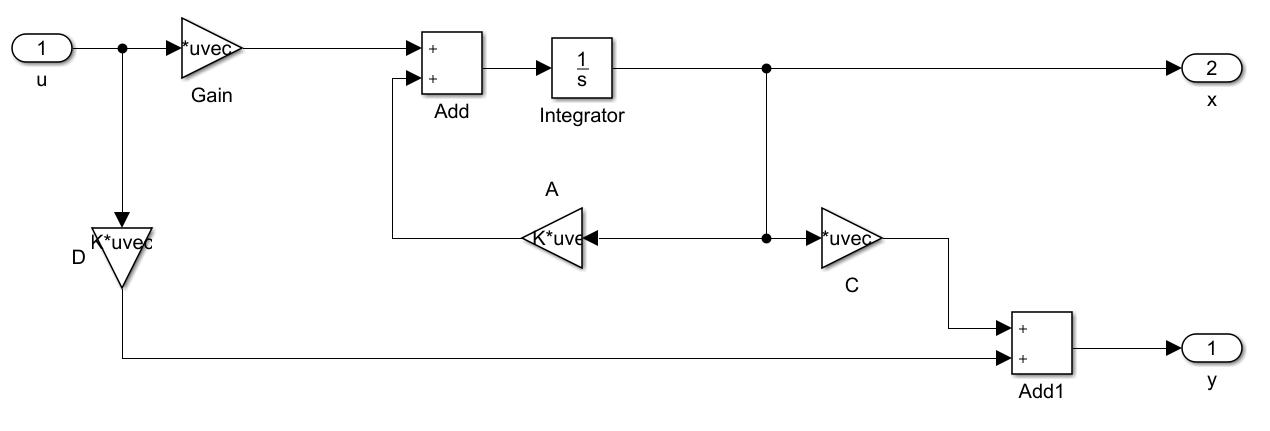
\includegraphics[width=\textwidth]{./part3_LQR2/not_generated/simulink_lin_sys.png}
			\caption{linear system}
			\label{fig: simulink diagram lin system LQR2}
		\end{subfigure}
		\caption{simulink diagrams}
	\end{figure}

\subsection{Simulation with noise}
	A first approach to the simulation($f_c=2Hz$) with noise is to try out some parameters and see what happens. A reasonable amount of noise seems to be with a noise of power=$10^{-8}$. If the noise is much higher then this, then controlling the process becomes very hard. The results of these simulations are displayed in figure~\ref{fig:simulation results with a noise with power=$10^{-8}$}. As this is not a very scientific way of simulating, no real conclusions can be made from these simulations.
	\begin{figure}[H]
		\centering
		\begin{subfigure}[b]{0.45\textwidth}
			\includegraphics[width=\textwidth]{./part3_LQR2/normal_parameters_estimated_states.png}
			\caption{estimated states}
		\end{subfigure}
		\begin{subfigure}[b]{0.45\textwidth}
			\includegraphics[width=\textwidth]{./part3_LQR2/normal_parameters_states.png}
			\caption{real states}
		\end{subfigure}
		\begin{subfigure}[b]{0.45\textwidth}
			\includegraphics[width=\textwidth]{./part3_LQR2/normal_parameters_input.png}
			\caption{input to motor}
		\end{subfigure}
		\caption{simulation results with a noise with power=$10^{-8}$}
		\label{fig:simulation results with a noise with power=$10^{-8}$}
	\end{figure}
\subsection{Simulation with noise estimated from experiments}
	A more scientific way of simulating with noise is to estimate the power of the noise from measurements. As explained in the next section, measurements where taking when the controller and motor where idle. These measurements contain very little to no model behavior and so contains mostly noise. $f_c$ was set to 2Hz and measurements where taken before and after the low pass filter in the estimator. 
	
	The variance of these measurements on $\alpha$ and $\theta$ where $1.96 \cdot 10^{-7}$ for $\alpha$ and $1.4 \cdot 10^{-6}$ for $\theta$. As the variance is the power in the signal ($power = \frac{u_{eff}^2}{R} = \frac{stdev^2}{1 \Omega}$= variance) there 2 values are taken for the simulation noise.
	
	The resulting simulations are displayed in figure~\ref{fig:LQR2 simulation with real noise} and are quiet pleasing. There seems no need to adjust Q and R even further. The initial guess of the noise seems to be quiet accurate even tough it was almost just a gamble. The problem that arise with the estimators is that there is overshoot and a longer settling time.
	\begin{figure}[H]
		\centering
		\begin{subfigure}[b]{0.45\textwidth}
			\includegraphics[width=\textwidth]{./part3_LQR2/noise_experiments_estimated_states.png}
			\caption{estimated states}
		\end{subfigure}
		\begin{subfigure}[b]{0.45\textwidth}
			\includegraphics[width=\textwidth]{./part3_LQR2/noise_experiments_states.png}
			\caption{real states}
		\end{subfigure}
		\begin{subfigure}[b]{0.45\textwidth}
			\includegraphics[width=\textwidth]{./part3_LQR2/noise_experiments_input.png}
			\caption{input to motor}
		\end{subfigure}
		\caption{simulation results with noise derived from experiments}
		\label{fig:LQR2 simulation with real noise}
	\end{figure}

\subsection{Investigating the role of the cut-off frequency}
Most of the noise is high frequency while the model dynamics are in the low frequency area. This offers an opportunity to get rid of most of the noise by filtering. A low-pass filter can keep the slow model dynamics and remove the high frequency noise. If the cut-off frequency of this filter is chosen too high then too much noise is allowed to get to the estimator and the controller output will contain a lot of noise (figure~\ref{fig:LQR2 simulation with real noise high noise}). If the cut-off frequency is chose too low then part of the model dynamics is filtered out. The controller will not be able to properly control the process as can be seen on figure~\ref{fig:LQR2 simulation with real noise low noise}.

\begin{figure}[H]
	\centering
	\begin{subfigure}[b]{0.45\textwidth}
		\includegraphics[width=\textwidth]{./part3_LQR2/noise_experiments_low_fc_estimated_states.png}
		\caption{estimated states}
	\end{subfigure}
%	\begin{subfigure}[b]{0.45\textwidth}
%		\includegraphics[width=\textwidth]{./part3_LQR2/noise_experiments_low_fc_states.png}
%		\caption{real states}
%	\end{subfigure}
	\begin{subfigure}[b]{0.45\textwidth}
		\includegraphics[width=\textwidth]{./part3_LQR2/noise_experiments_low_fc_input.png}
		\caption{input to motor}
	\end{subfigure}
	\caption{simulation results with noise derived from experiments, $f_c=0.5Hz$}
	\label{fig:LQR2 simulation with real noise low noise}
\end{figure}

\begin{figure}[H]
	\centering
	\begin{subfigure}[b]{0.45\textwidth}
		\includegraphics[width=\textwidth]{./part3_LQR2/noise_experiments_high_fc_estimated_states.png}
		\caption{estimated states}
	\end{subfigure}
%	\begin{subfigure}[b]{0.45\textwidth}
%		\includegraphics[width=\textwidth]{./part3_LQR2/noise_experiments_high_fc_states.png}
%		\caption{real states}
%	\end{subfigure}
	\begin{subfigure}[b]{0.45\textwidth}
		\includegraphics[width=\textwidth]{./part3_LQR2/noise_experiments_high_fc_input.png}
		\caption{input to motor}
	\end{subfigure}
	\caption{simulation results with noise derived from experiments, $f_c=10Hz$}
	\label{fig:LQR2 simulation with real noise high noise}
\end{figure}
